\subsection{State of the Art}
I det følgende afsnit vil vi komme ind på diverse skemalægningsværktøjer, samt nogle algoritmer som kan bruges indenfor dette område
\label{sota}

\subsubsection{Udenlandske skemalægningsværktøjer}
Indenfor skemalægning findes allerede nogle løsninger på de udfordringer, som kan opstå indenfor skemalægning. En af disse er USA Schedulers' program ved navn School Master Scheduling Software\cite{USAS}. Dette er et program, som først og fremmest tager de studerende i betragtning. Programmet er i stand til at lave funktionelle skemaer ud fra de studerenes ønsker og analysere de mest optimale løsninger ud fra ønskerne, og ud fra dette undgå konflikter såsom to moduler, der ligger samtidigt. Ud fra dette kan programmet så vise, at studerende der deltager aktivt i begge, bliver nødt til at vælge den ene fra.
\begin{figure}[h!]
	\centering
	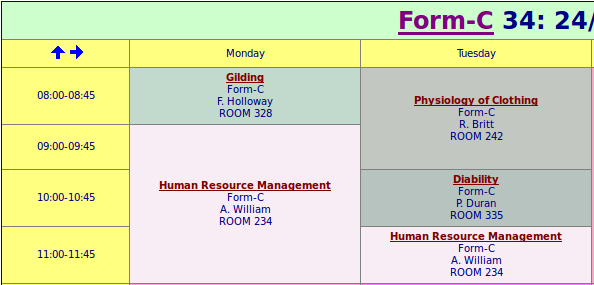
\includegraphics[width=1.0\textwidth]{../Billeder/MimosaSoftware.png}
	\caption{Udsnit af Mimosa Scheduling Software\cite{mimosaPicture}}
	\label{fig:Mimosa}
\end{figure}
\FloatBarrier
Et andet stykke software, ved navn Mimosa Scheduling Software\cite{Mimosa}, (se figur \ref{fig:Mimosa}), fokuserer mere på de grundlæggende udfordringer såsom overbooking og at gøre det nemmere at kunne ændre på skemaerne, hvis der skulle opstå en uventet udfordring. Programmet er i stand til at lave skemaer for lærere, elever, klasser og lokaler, altså alt det som enhver dansk folkeskole har brug for. Institutionerne henter programmet, laver deres egne ressourcer, hvilket vil sige lærere, elever, lokaler osv. og fordeler derefter disse ud over dagene. Programmet vil så fortælle, om dette kan lade sig gøre, og hvis det ikke er tilfældet, vil det fortælle hvorfor\cite{MimosaTutorial}. I modsætning til School Master Scheduling, er Mimosas program mere henvendt til skemalæggerne og ikke så meget til de studerende. 

Begge programmer løser dog så at sige ikke selve skemalægningsopgaven, da dette stadig gøres manuelt af skemalæggeren eller de individuelle studerende for deres eget skema, men fungerer i stedet som et kontrollerende led. Ser man på de 10 mest anbefalede skemalægningsprogrammer fra hjemmesiden TopTenReviews\cite{top10Schedulers}, er de ikke rangeret ud fra automatisk skemalægning. Programmet som kommer tættest på, vil være Auto-Scheduler, men denne funktionalitet virker kun for medarbejdere ud fra en historik og er derfor ikke automatisk skemalægning. Besøger man et af de ti anmeldte programmers hjemmesider, finder man ingen information omkring programmernes evner indenfor dette. Et program som vil være i stand til helt automatisk at lave skemaer til alle på for eksempel en dansk folkeskole, udelukkende ud fra information om de ansatte, eleverne og tilgængelige klasselokaler, vil derfor være innovativt og nyttigt. Disse top-ti skemalægningsværktøjer er også mest henvendt til firmaer, så firmaerne kan tildele hver lønmodtager arbejdsopgaver og holde styr på, hvor meget løn hver lønmodtager får, hvilket er noget anmeldelsesiden går meget op i og bedømmer skemalægningsværktøjerne ud fra.

\subsubsection{Tabulex}
\begin{figure}[h!]
	\centering
	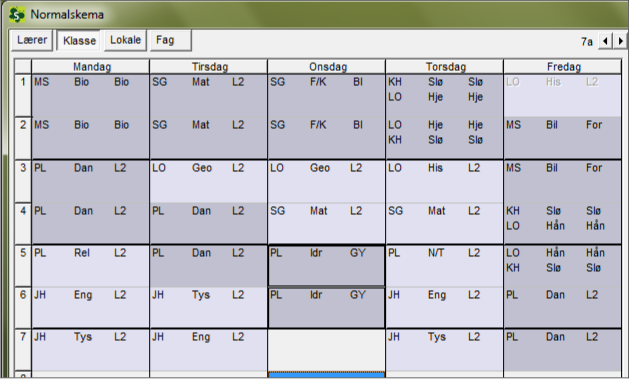
\includegraphics[width=1.0\textwidth]{../Billeder/TabulexPicture.png}
	\caption{Tabulex skemalægningsprogram\cite{Tabulex}}
	\label{fig:TabulexPicture}
\end{figure}
\FloatBarrier
På Tingstrup skole vil et program ved navn Tabulex (se figur \ref{fig:TabulexPicture}) blive taget i brug i forbindelse med skemalægningen. Det er et skemalægningsværktøj, der som de forrige kræver, at brugeren stiller programmet en hel del krav, heriblandt hvordan lærerens tid skal prioriteres, hvornår lektionerne lægges, og hvor meget hver af disse regler skal prioriteres og overholdes af programmet\cite{Tabulex}. Tabulex kan selv forsøge i bedste fald at lægge et skema ud fra de mange begrænsninger, som skemalæggeren har stillet, og undervejs vil programmet informere brugeren, hvis kravene som er opstillet ikke muliggør et skema, og man kan rette dem til. Herefter er det  muligt at fortsætte skemalægningen eller starte lægningen forfra. Ligesom de andre skemalægningsværktøjer, kommer det med en grafisk brugerflade, som understøtter drag\&drop, og som er rimeligt overskuelig. Tabulex kan dog ikke holde styr på regnskabet ligesom værktøjerne i forhenværende afsnit, men dette er heller ikke hvad programmet er lavet til at håndtere. Det bør nævnes, at Tabulex har en dybdegående dokumentation omkring hvordan programmet eksporterer til en CSV-fil\cite{Tabulex_csv}, og da et af kravene stillet af vores case er, at det endelige skema skal kunne inddrages i SkoleIntra, KMD Elev og andre programmer\cite{interview_Kaerby}, som netop tager imod CSV-formatet (se figur \ref{fig:kompatibleFiltyper}), er dette noget, vi vil kigge nærmere på.
\begin{figure}[h!]
	\centering
	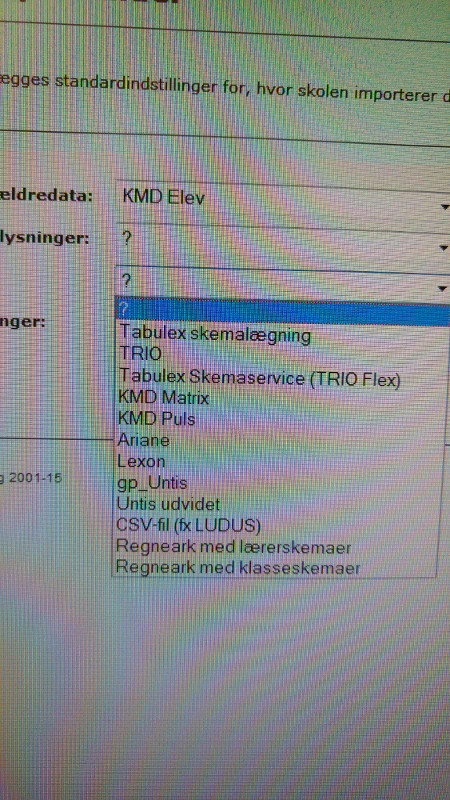
\includegraphics[width=0.4\textwidth]{../Billeder/Skemaimportering_filtyper_Intra.jpg}
	\caption{Skolens online system SkoleIntra kan læse forskellige filformater}
	\label{fig:kompatibleFiltyper}
\end{figure}
\FloatBarrier
\subsubsection{KMD Educa}
Et andet program Tingstrup-skolen bruger er KMD Educa, hvilket er en samling af forskellige værktøjer\cite{KMD}, der gør det muligt blandt andet at vikarføre, lægge skemaer og håndtere karakterresultater for den enkelte elev, som går på skolen eller har gået på skolen. Dette er en af de mange grunde til, at Aalborg Kommune har valgt at benytte sig af KMD Educa programmet ``Elev''\cite{useCase_KMD_Educa_Elev}.

\subsubsection{Docendo}
Vores case, Kærbyskolen, brugte et program ved navn Docendo før skolestart 2015, men selvom firmaet selv giver udtryk for, at deres program er meget fleksibelt\cite{Docendo}, var det ikke fleksibelt nok for skolen, og de valgte derfor at lægge skema manuelt. Programmet tillader at lægge skemaet elektronisk, lave varierende lektionslængde og tælle brugte timer, så eleverne hverken får for lidt lektioner, eller alt for mange. Ud fra deres video\cite{Docendo_video}, er det nemt at gå til; klasserne kan holdes styr på i en grafisk brugerflade, lektionerne kan flyttes rundt som det passer en, og hvis man gør dette, ændres tidspunktet i lektionsrubrikken også. Skemaet lægges dog for hver uge, men dette er i sidste ende ligegyldigt, da den tidligere uges skema godt kan genbruges.

\subsubsection{Untis}
Untis er et af de mest anvendte skemalægningsprogrammer i Europa. Untis skriver, at deres program kan bruges af alle og har funktionerne til at gøre skemalægningen nem og overskuelig for skemalæggeren. Nogle af mulighederne med Untis er fuldautomatisk skemaoptimering med en hurtig optimeringsalgortime og at det er egnet til alle skoletyper.\cite{UntisDK}
Untis har et brugervenligt system, hvor man indtaster skolens specifikke oplysninger, og ud fra oplysningerne kan Untis danne et skema til skolen baseret på skolens krav og hvad skolen lægger mest vægt på, for eksempel om der må være det samme fag to dage i træk. På figur \ref{fig:untisskema} ses, at Untis har et fleksibelt skemalægningssystem, hvor der kan ændres i flere variable baseret på skolens interesser. 
\begin{figure}[h!]
	\centering
	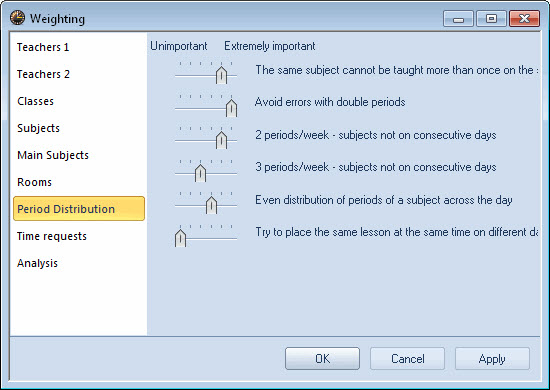
\includegraphics[width=0.7\textwidth]{../Billeder/untisskema.jpg}
	\captionsource{Untis fleksible skemalægningssystem}{\url{http://www.school-timetabling.com/content/images/UK/weighting.jpg}}
	\label{fig:untisskema}
\end{figure}
\FloatBarrier
Algoritmen Untis bruger, giver flere resultater, hvor man selv kan bestemme om skemaet passer til ens behov. Når skemaet er blevet lagt, er der flere muligheder for hvordan det kan blive vist frem.\cite{UntisInt}

\subsubsection{Brute Force}
Vi vil nu undersøge nogle af de teknologier, som et program kunne benytte sig af for at finde frem til et skema. Den mest systematiske løsning, og måske den løsning der er nemmest af gå til, er brute force-metoden. Brute force går som navnet antyder ud på at bruge rå kraft for at finde løsningen. Måden dette gøres på i en computer, er ved at prøve samtlige muligheder, indtil man når det ønskede resultat.

I forhold til skemalægning, ville man altså forsøge samtlige sammensætninger af moduler i løbet af ugen, for alle klasse. For at undersøge om dette ville virke, kan vi regne ud hvor mange skemaer et program maksimalt ville skulle teste.

$$ (\text{UgentligeModuler})! \times \text{AntalKlasser} = \text{AntalSkemaer}$$

Hvis vi indsætter informationer fra Kærbyskolen som har 12 klasser og 10 lektioner om dagen får vi følgende antal skemaer:
$$ (10\cdot 5)! \cdot 12 = 3,65\cdot 10^{65} $$

Som det kan ses ud fra det enorme tal vi lige har regnet ud, er det umuligt at tjekke samtlige skemaer, for at finde det bedste, og man må derfor nøjes med at finde de første $n$ skemaer ved hjælp af bruteforce. Da man som regel kun ændrer \'en ting af gangen når man brute-forcer, kunne disse $n$ skemaer dog komme til at ligne hinanden meget, og man får ikke stor variation i skemaet.

\subsubsection{Heuristisk metode}
Ordet heuristisk bliver i ordbogen defineret som ``vedr. erkendelse af ny viden, opnået fx ved systematisk søgning efter information eller afprøvning af muligheder''\cite{Ordnet}.

\subsubsection{Monte Carlo / Las Vegas}

\subsubsection{Genetiske algoritmer}

